\section{Modeling, Simulation, and Experimental Optimization}

In order to create an experimental optimization plan for the project, first, the hardware and software constraints of the problem were identified. Since a different set of constraints can be applied based on the use-case, different models for each set of constraints were created. Finally, simulations were run on the generated models in order to analyze and understand what parts of the project to optimize through experimentation. The details of the code written for modeling and simulation can be found in Appendix \ref{sec:appendix-for-code}.

\begin{figure}[H]
    \centering
    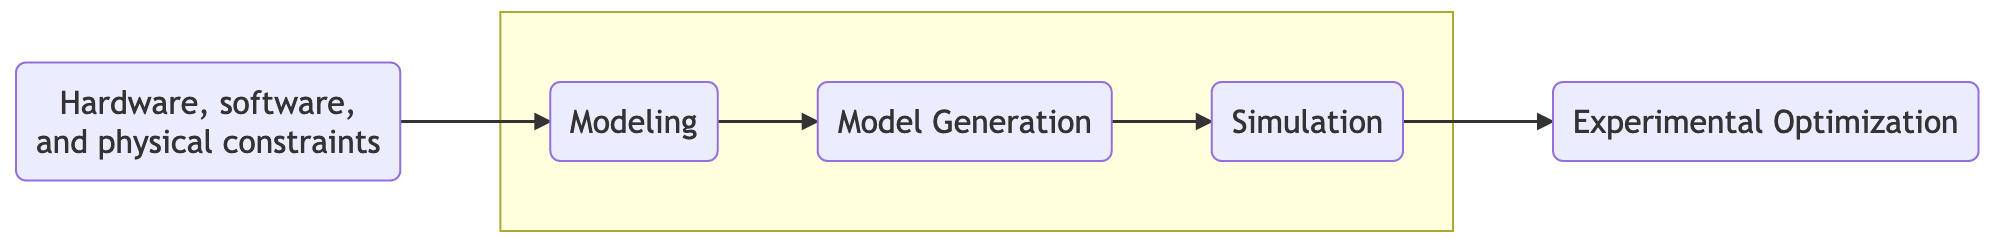
\includegraphics[width=0.95\textwidth]{images/mod_sim_flowchart.png}
    \caption{The high level flowchart capturing the modeling, simulation, and optimization process}
    \label{fig:mod-sim-flowchart}
% graph LR
%   model(Modeling)
%   modgen(Model Generation)
%   sim(Simulation)
%   opt(Experimental Optimization)
%   const(Hardware, software, <br> and physical constraints)

%   const --> model
%   subgraph " "
%     model --> modgen
%     modgen --> sim
%   end
%   sim --> opt
\end{figure}

%%%%%%%%%%%%%%%%%%%%%%%%%%%%%%%%%%%%%%%%%%
\subsection{Modeling}
The modeling was focused on hub-spoke and mesh networks. In each of the created models, each node represents the ESP8266 microcontroller-based physical devices, while the connections between the nodes represent the IEEE 802.11 based wireless communication. 

% Since the final design depends on the physical space, hardware, and software constraints of the project, the model was constructed with these constraints into consideration.%

According to our model, any two devices can only communicate if there is an established communication between them, and they are within each other's communication range. This models how wireless devices communicate with each other in the physical world. Given that the ESP8266 microcontrollers' built-in IEEE 802.11 based WiFi modules can typically connect with distances up to 100m \cite{chabukswardesign}, this is how we set the communication ranges for the nodes in our models.

Further, the number of simultaneous connections per device is also dependent on the hardware and software limitations. Since the ESP8266 microcontroller-based devices can have a maximum of eight simultaneous wireless connections \cite{ESP8266_NONOS_V1_1_0_Release_Notes}, the connection limit per node in our models follows this constraint as well. To achieve this, our model allows a maximum of four connections.

Although using regular nodes is enough to create a mesh network, there need to be "hubs" in order to create a hub-spoke network topology. The hubs were modeled as special nodes that can handle a larger number of simultaneous connections in the network. It was also assumed that the hubs are connected to each other with low-latency and high-speed communication mediums, as is often the case in a typical home network where routers are connected in this manner. 

In using the aforementioned "nodes" and "hubs", different network models were generated to represent various real-life network conditions. The next subsection explains how these models are generated.


%%%%%%%%%%%%%%%%%%%%%%%%%%%%%%%%%%%%%%%%%%
\newpage
\subsection{Model Generation}
\label{model-gen-section}
First, a two-dimensional rectangular virtual space was created based on the physical space constraints. The virtual space was configured to be flexible in terms of dimensions to accommodate different physical space requirements. Later, the target number of nodes were placed into the virtual space randomly using Python's \cc{randint()} method in order to prevent possible biases, as shown in \ref{fig:modeling_node}.

\begin{figure}[H]
    \centering
    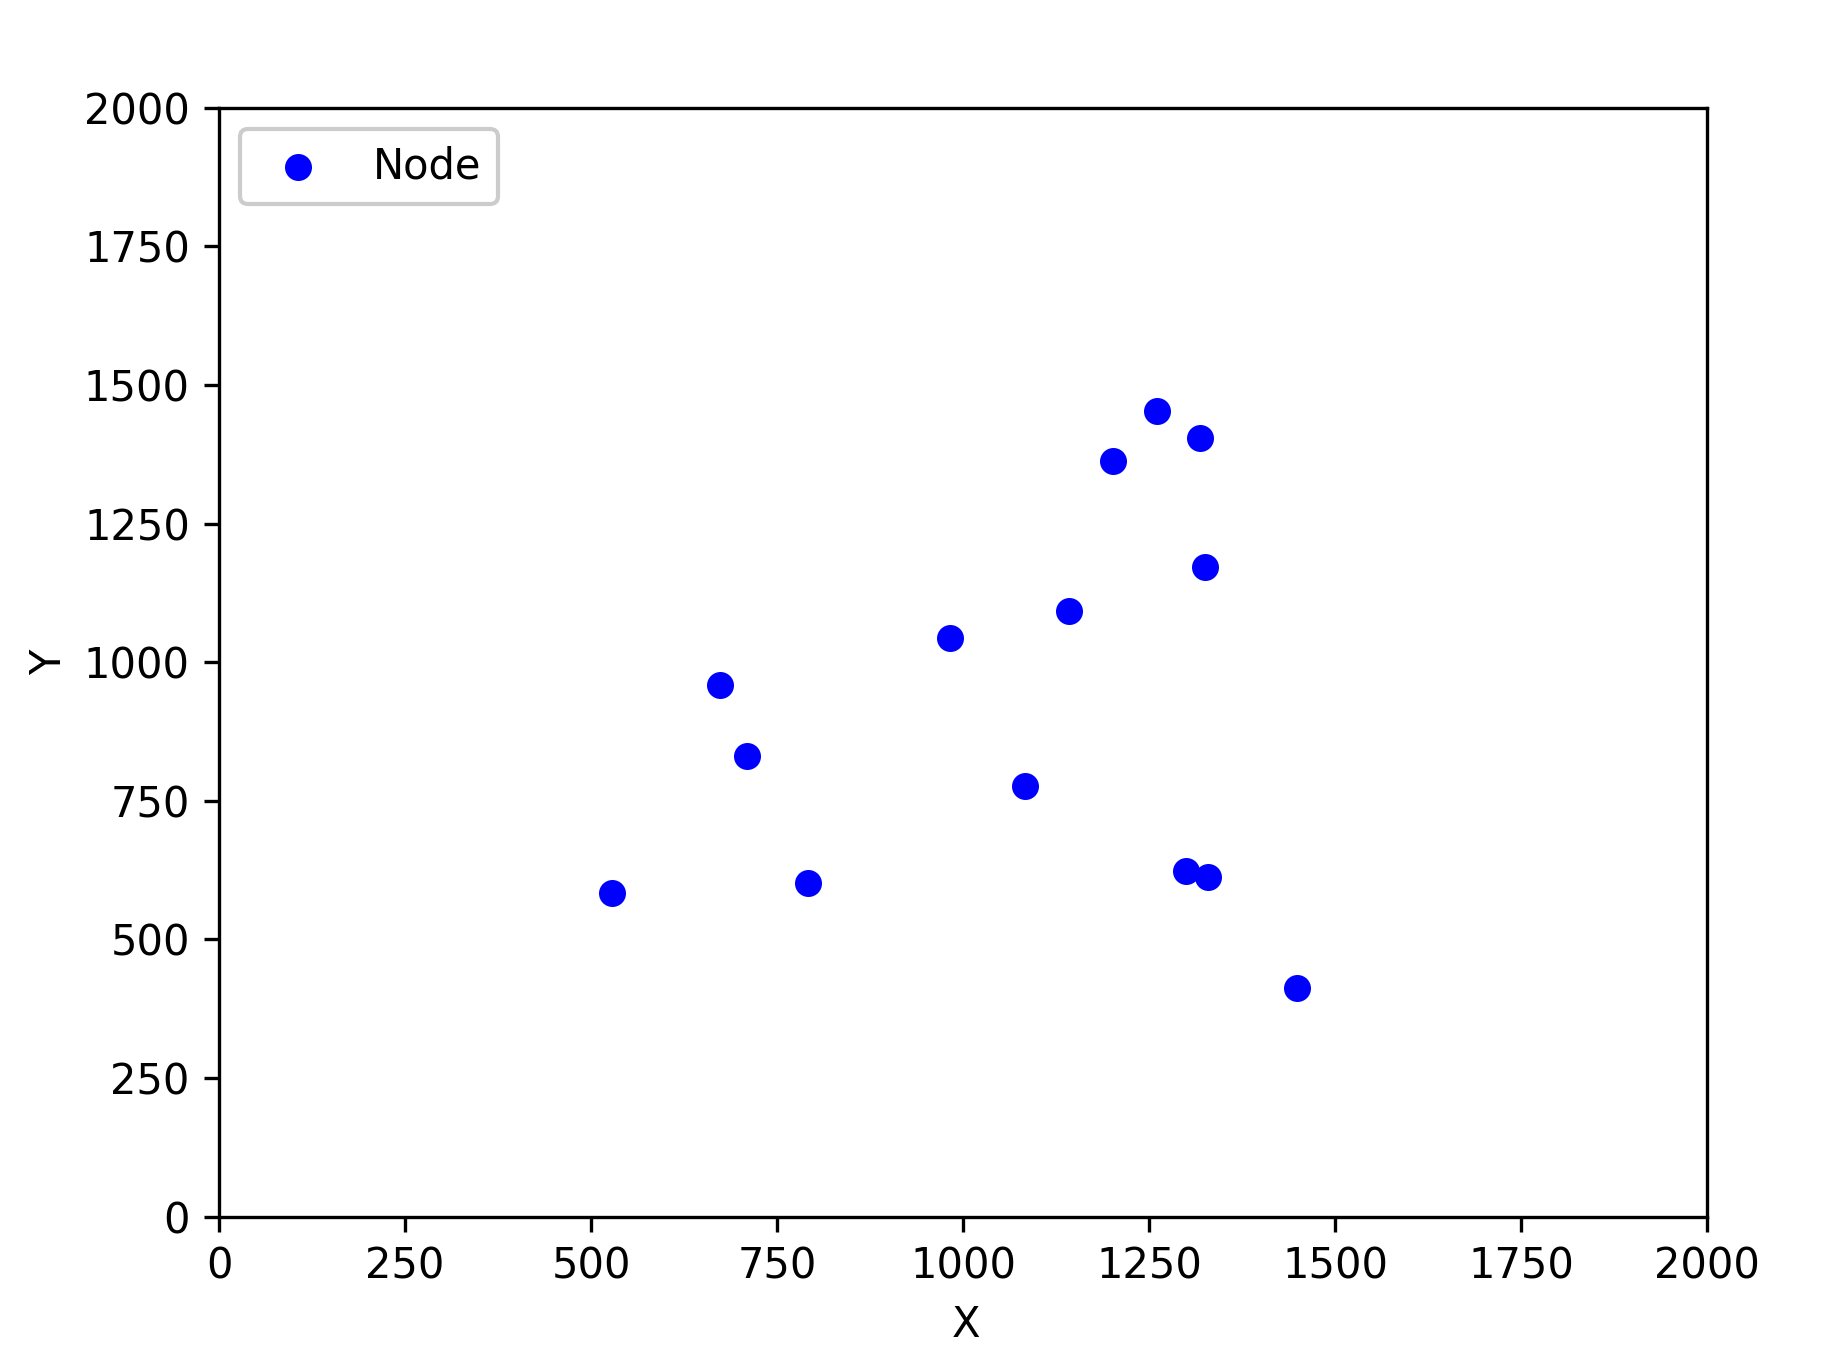
\includegraphics[width=0.42\columnwidth]{images/modeling_nodes_only.png}
    \caption{Nodes randomly distributed in the virtual space}
    \label{fig:modeling_node}
\end{figure}


Once the placement was completed in Figure \ref{fig:modeling_node}, the communication range of each node was determined within the virtual space, as shown in Figure \ref{fig:modeling_mesh}. Based on the simultaneous connection budget available for each node and overlapping communication ranges, the connections between the nodes can be created to construct a mesh network, as shown in Figure \ref{fig:modeling_mesh}.

\begin{figure}[H]
    \centering
    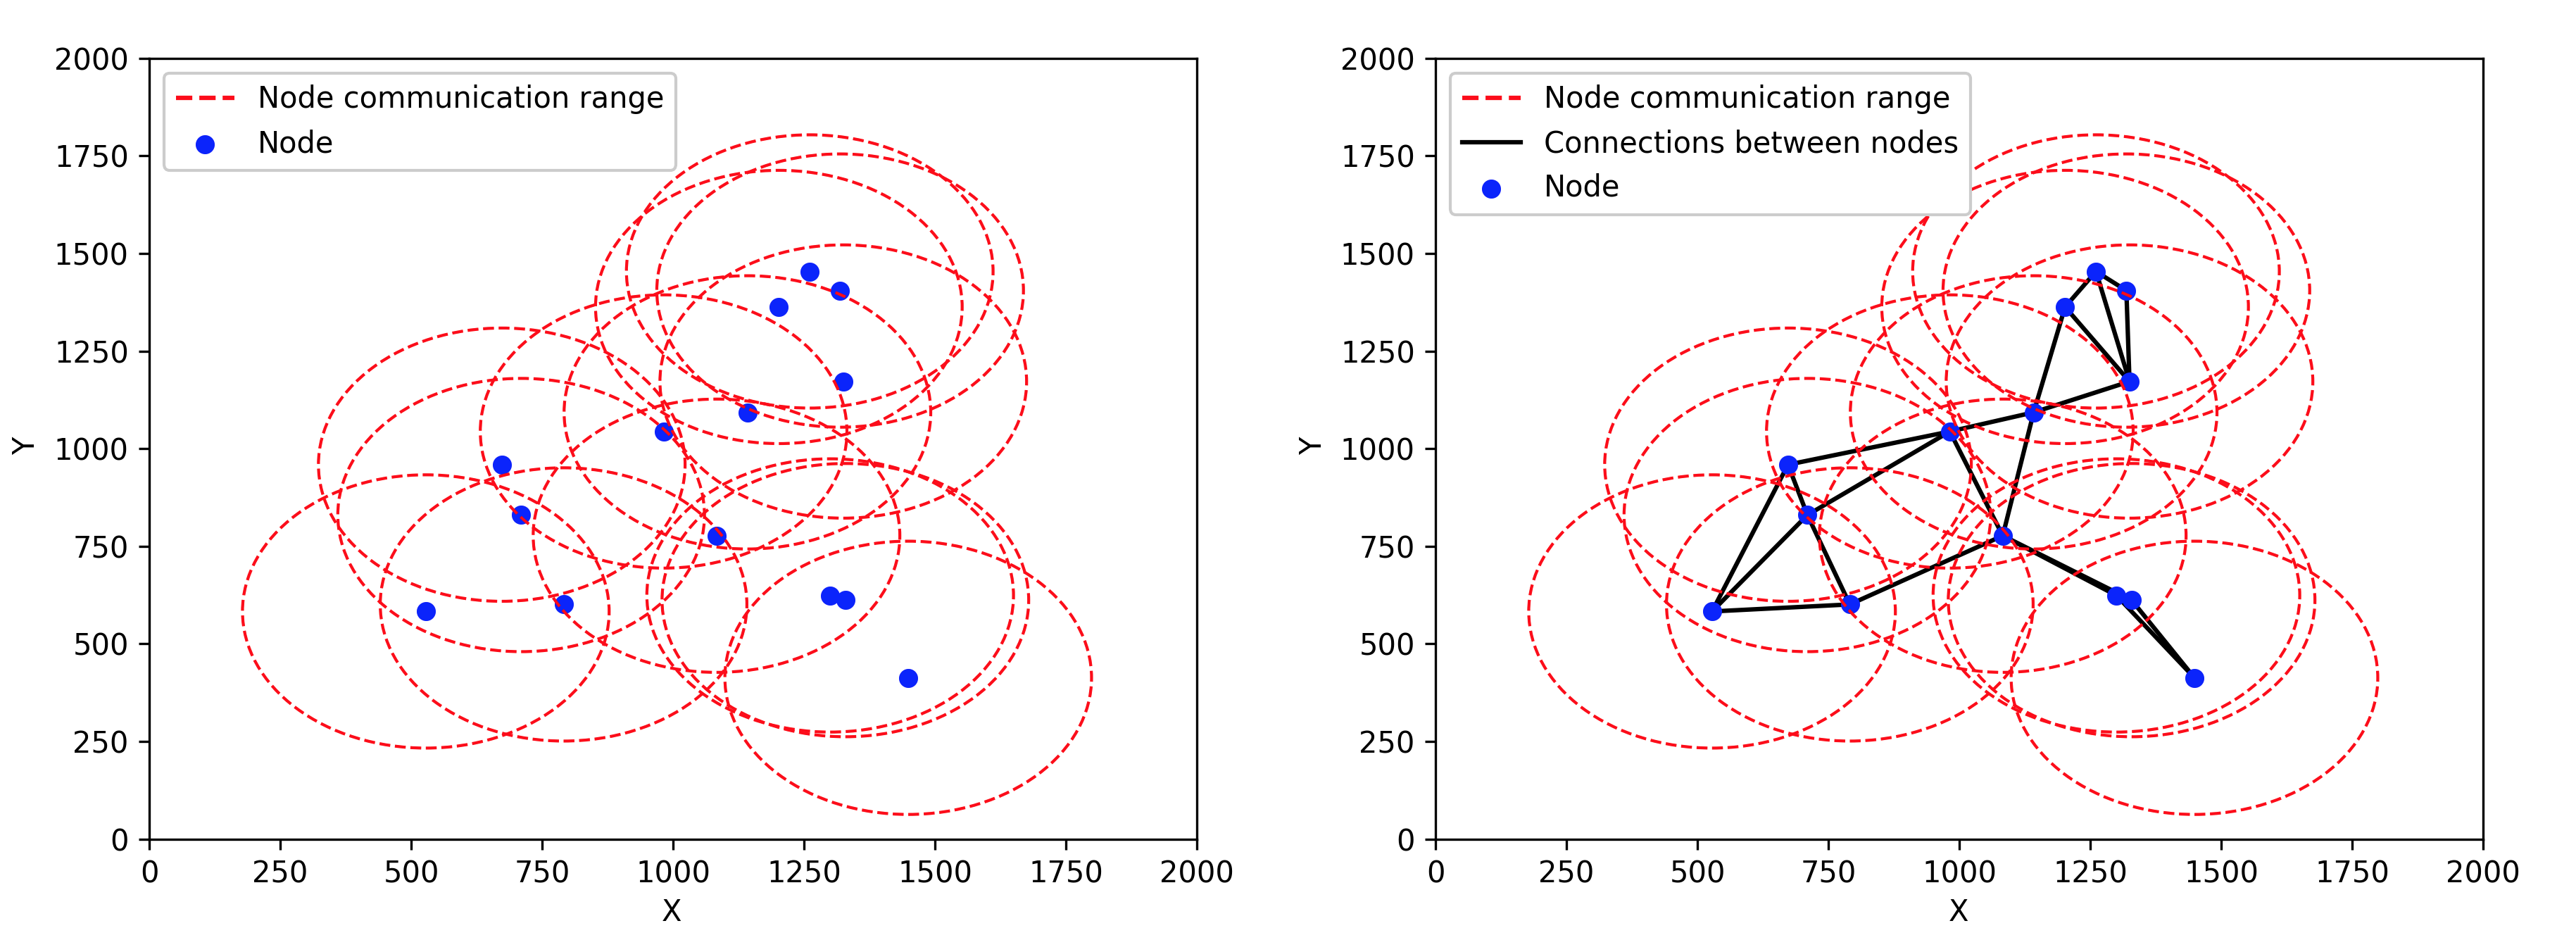
\includegraphics[width=0.88\columnwidth]{images/modeling_mesh.png}
    \caption{Left: Nodes and their communication ranges, Right: Nodes connected in mesh network topology based on the communication ranges}
    \label{fig:modeling_mesh}
\end{figure}

A hub-spoke network was also created from the random node placement shown in Figure \ref{fig:modeling_node}. However, it was not enough to simply check for the connection budget and overlapping communication ranges to construct a hub-spoke network topology, as was done for the mesh network. The nodes must communicate with each other via hubs. In order to find the optimal placement of the hubs for the created network, the "k-means" algorithm was applied iteratively until the created group of nodes covered the entire network. Next, a hub was placed at the center of each group, as shown on the left in Figure \ref{fig:modeling_star}. Nodes were then connected to the hubs, as shown on the right in Figure \ref{fig:modeling_star}.

\begin{figure}[H]
    \centering
    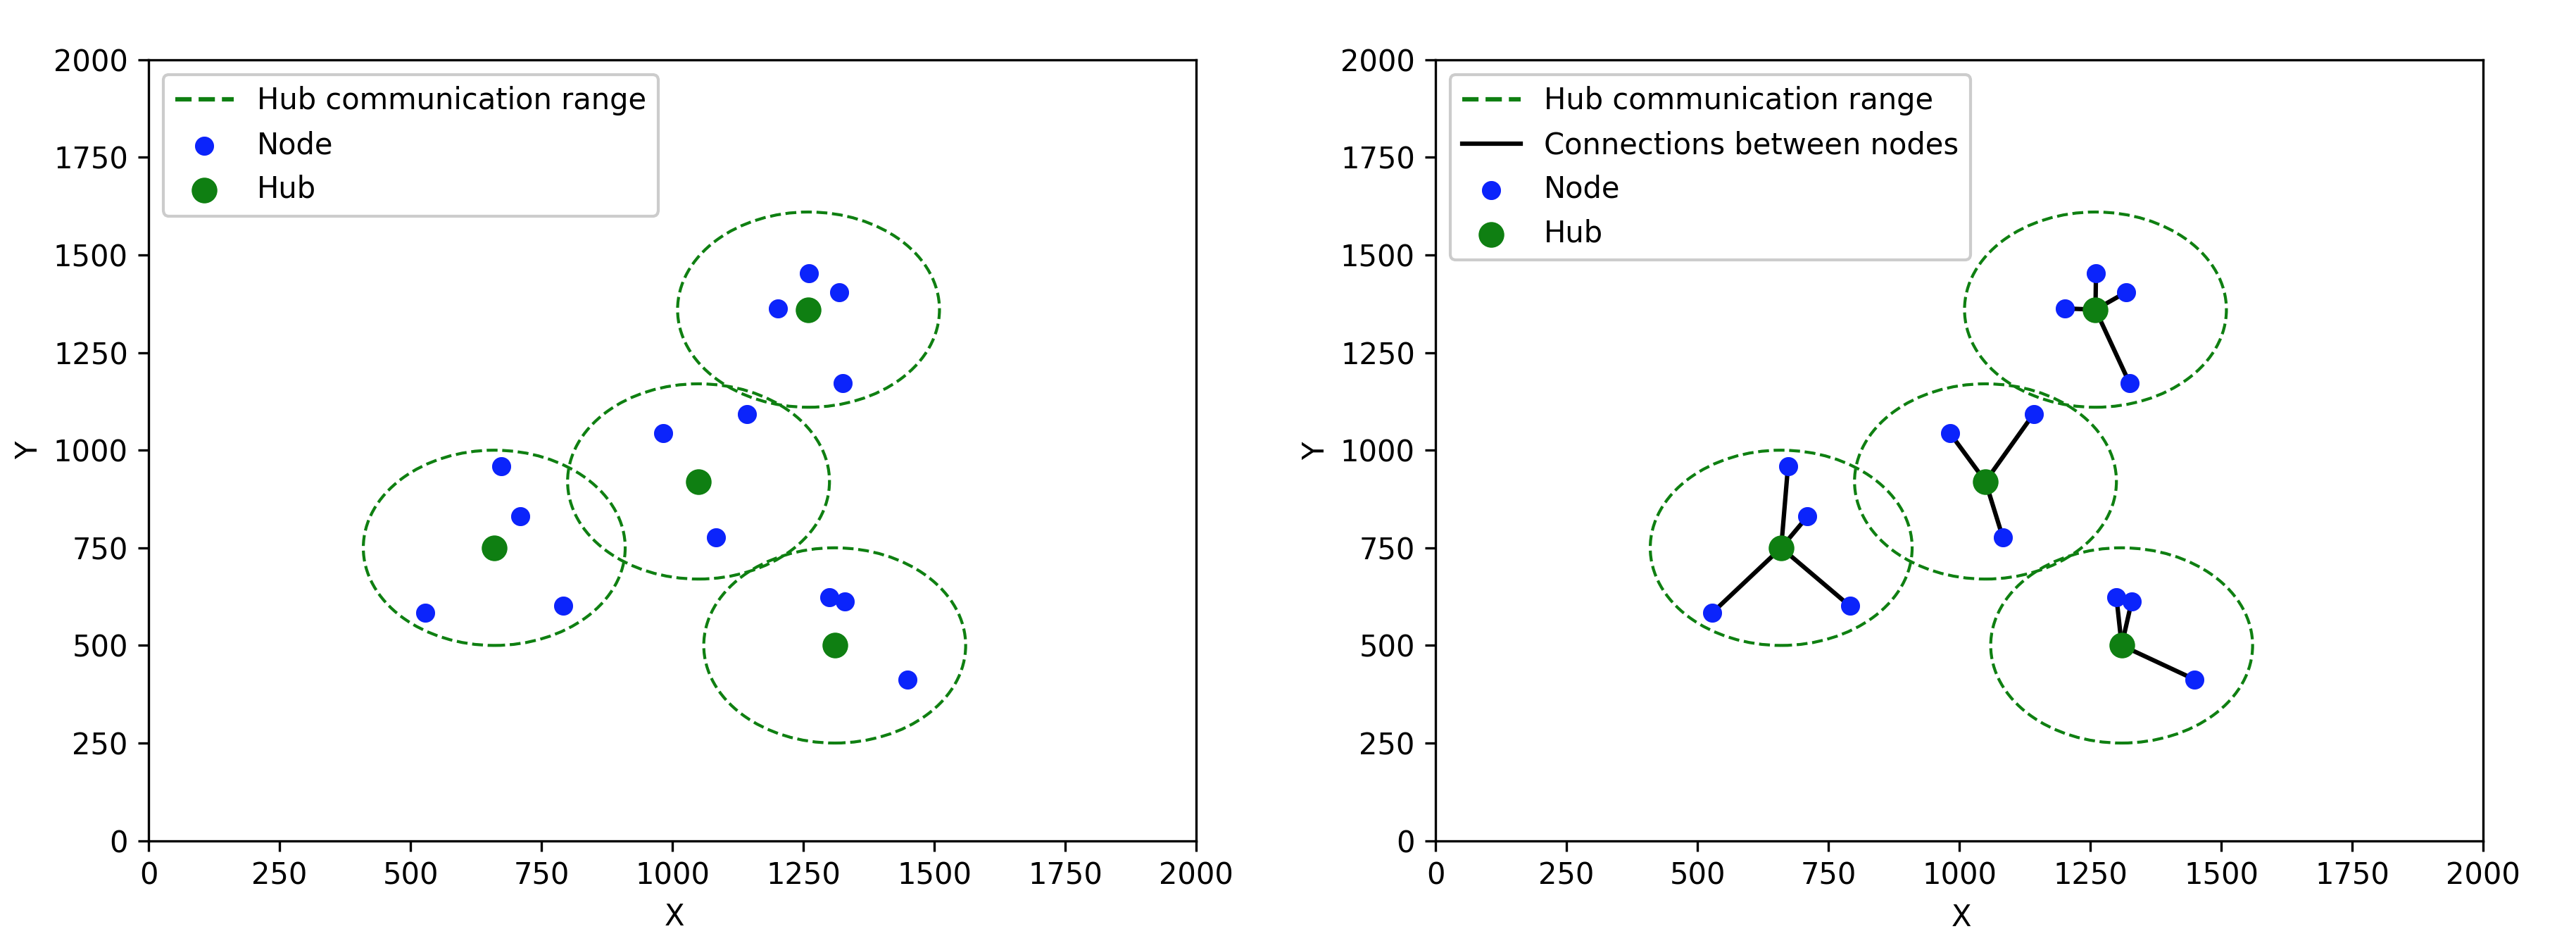
\includegraphics[width=0.88\columnwidth]{images/modeling_star.png}
    \caption{Left: Grouped nodes and corresponding hubs, Right: Nodes connected in hub-spoke (star) network topology based on the communication ranges}
    \label{fig:modeling_star}
\end{figure}

Figure \ref{fig:modeling_complex} demonstrates that the node placement process can be repeated with a greater number of nodes, different communication ranges \& budgets to create more complex hub-spoke and mesh networks
\begin{figure}[H]
    \centering
    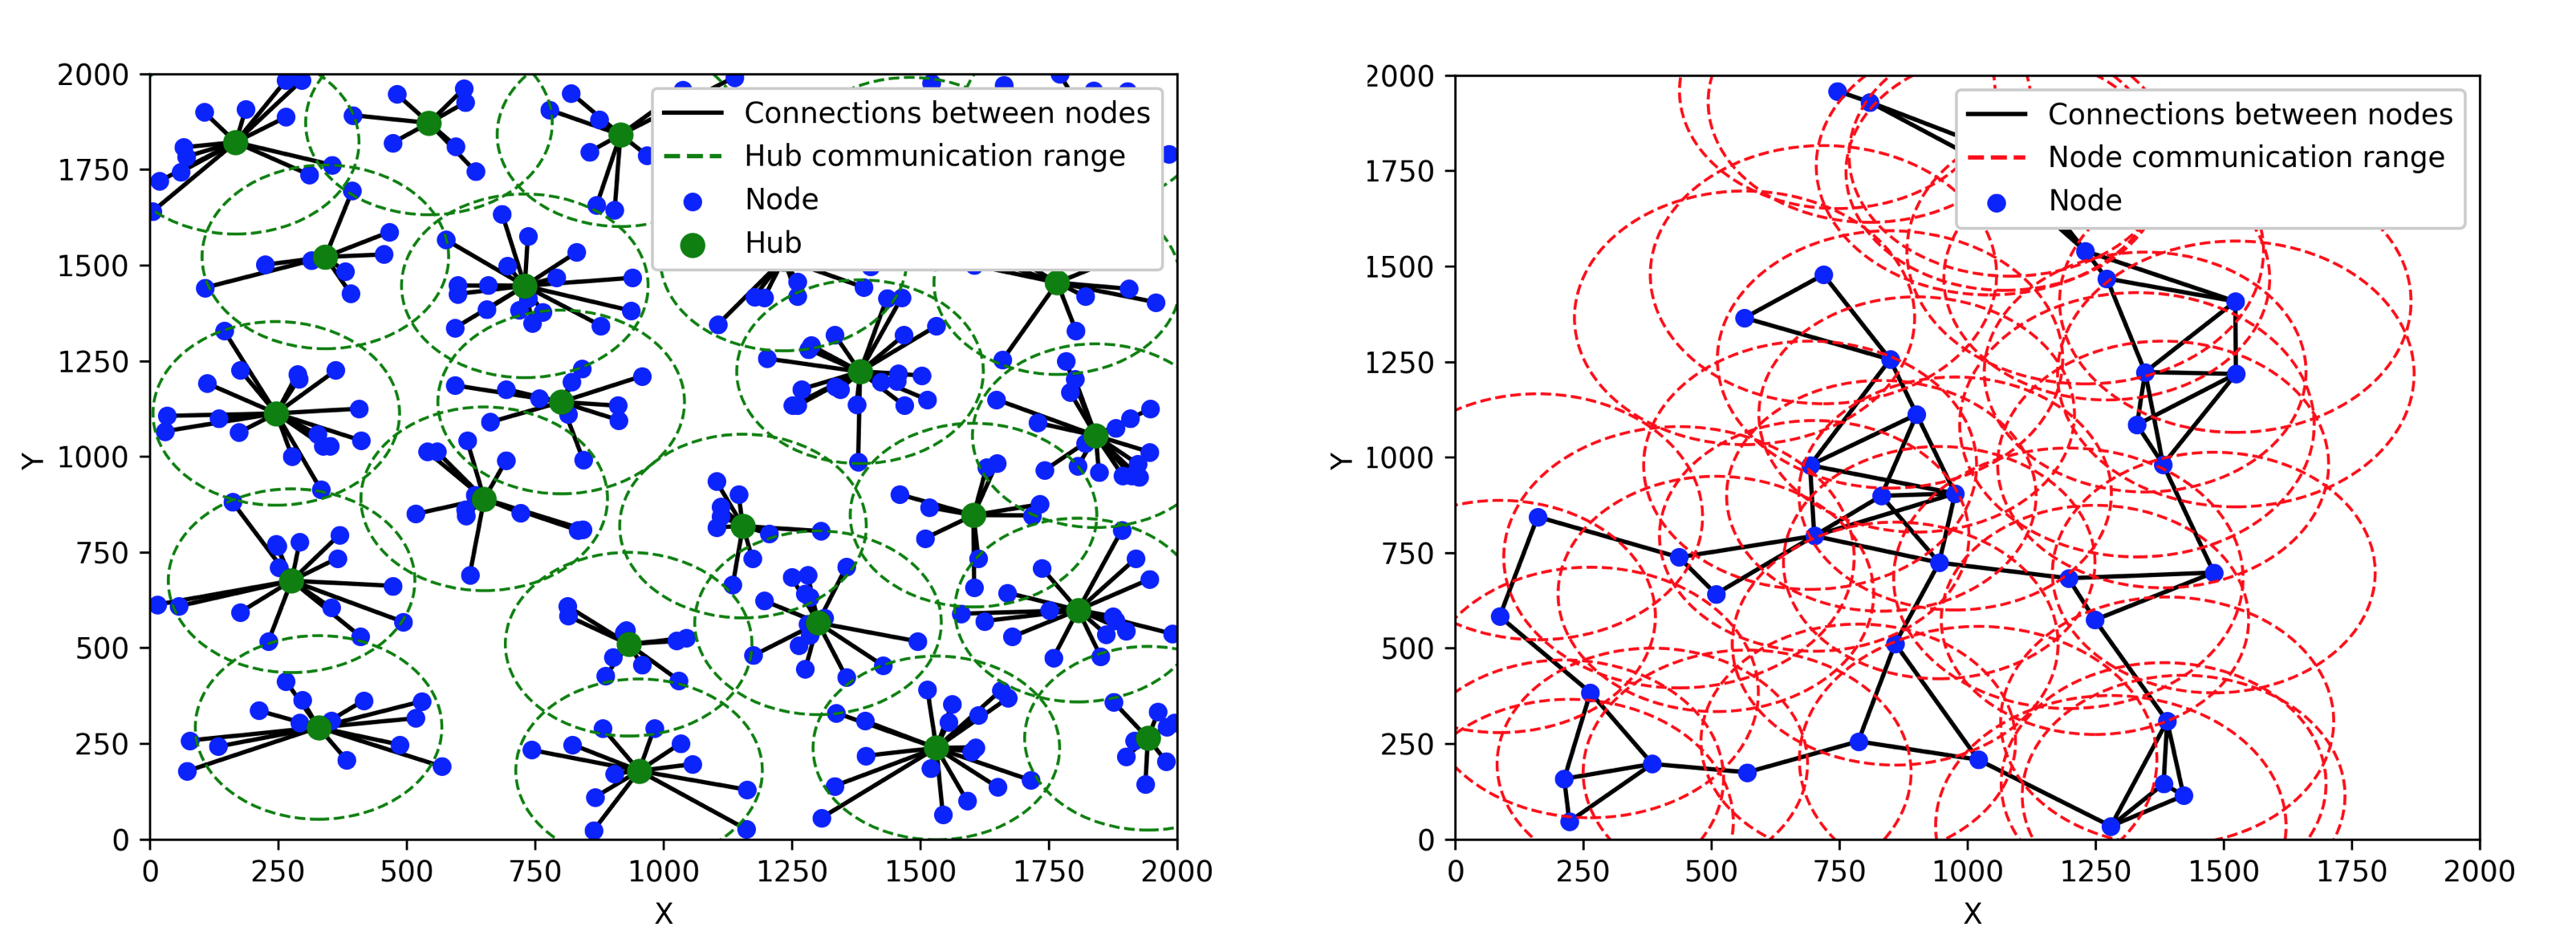
\includegraphics[width=0.88\columnwidth]{images/modeling_complex_unified.png}
    \caption{Left: Hub-spoke (star) network topology created in the virtual space, Right: Mesh network topology created in the virtual space}
    \label{fig:modeling_complex}
\end{figure}

The constructed models and the relations between the nodes and hubs in these models were exported for network communication simulations.

% talk about using python script to output x, y, z parameters (refer to it as \cc{network_generator} script)



%%%%%%%%%%%%%%%%%%%%%%%%%%%%%%%%%%%%%%%%%%
\subsection{Simulation and Experimental Results}

\subsubsection{Coracle Simulation}

We identified Coracle \cite{Coracle} as a tool to simulate the Raft consensus algorithm on heterogeneous networks. Coracle is a simulation framework written in the OCaml programming language, designed to evaluate "distributed consensus algorithms in settings that more accurately represent realistic deployments" \cite{howardCoracleEvaluatingConsensus2015}. The framework allows users to configure nodes, links, and events. 

A node can be defined as a hub, server, or client. From experimentation with the framework, we have learned that in the case of a server node, the node acts as a participant and carries out the responsibilities of a typical node, such as voting and log replication. When a node is configured as a hub, it foregoes its responsibility as a participant and acts as a router in the network. Finally, a client node is responsible for generating network traffic within the network between other clients \cite{howardCoracleEvaluatingConsensus2015}. Using the models generated, as described in section \ref{model-gen-section}, we set the routers in the hub-spoke topology to be hubs and set the remaining nodes to be servers. In the special case of a mesh topology, the nodes had to perform the role of a server and a hub simultaneously. Since Coracle does not allow for a node to hold two roles, we split each modeled node into two nodes: a hub node that maintained the modeled mesh connections and a server node that handled consensus actions. This way, we were able to emulate each node as having a very limited routing capability (maximum four connections), as is the case with ESP8266 chips.

In Coracle, links can either be unidirectional or bidirectional; moreover, multiple links between two nodes can exist. Essentially, this allows for the freedom to simulate whether a pair of nodes have half-duplex or full-duplex communication. Furthermore, each link can be assigned a latency category, small, medium, or large, to affect the package delivery time from source to destination nodes. \cite{howardCoracleEvaluatingConsensus2015}. For the sake of simplicity in our simulations, we modeled each link to have a small latency.

Events allow for nodes and links to activate or deactivate at user-defined timestamps. This can simulate unstable networks with multiple unreliable links that periodically fail. Moreover, considering real-world networks, this parameter can also be used to simulate the addition of new nodes into the network, with the only limitation being that node links would be predetermined \cite{howardCoracleEvaluatingConsensus2015}. To test the recovery ability between mesh and hub-spoke networks, we added a \cc{down hub time} parameter that brought down a random router in the network at the specified time. 

A limitation in the modeling and simulation workflow is the lack of traveling nodes, which rebuild their links based on available nearby nodes. However, we were able to test this with our library.

Coracle accepts a JavaScript Object Notation (JSON) file with a specific structure as an input. We wrote a \cc{simulation\_configuration} script to process the generated network models described in Section \ref{model-gen-section} and generate a JSON file based on the network parameters. Next, we wrote a \cc{run\_coracle} script to feed the generated JSON file into Coracle and gather the results. Finally, we wrote a \cc{experiment\_suite} script that generated multiple networks based on the desired number of nodes and area size, ran each network 100 times, and visualized these results.

\subsubsection{Results}
\label{sec:coracle_results}

Using Coracle, we were able to simulate several scenarios in order to justify the use of a mesh network in a consensus algorithm, as well as inform the configuration of our implementation. 

Figure \ref{fig:simulation_result_100} shows the results of a network simulation in a 10000 $unit^2$ area for both star and mesh topologies. The remaining graphs, which vary the number of nodes per area, can be found in Appendix \ref{sec:appendix-for-coracle-results}. In this scenario, the simulations ran for 1000 milliseconds each, and a random router was brought down for 200 milliseconds at the halfway mark (500 milliseconds). For each graph, we ran 100 simulations and gathered the generated statistics to inform our design.

\begin{figure}[H]
    \centering
    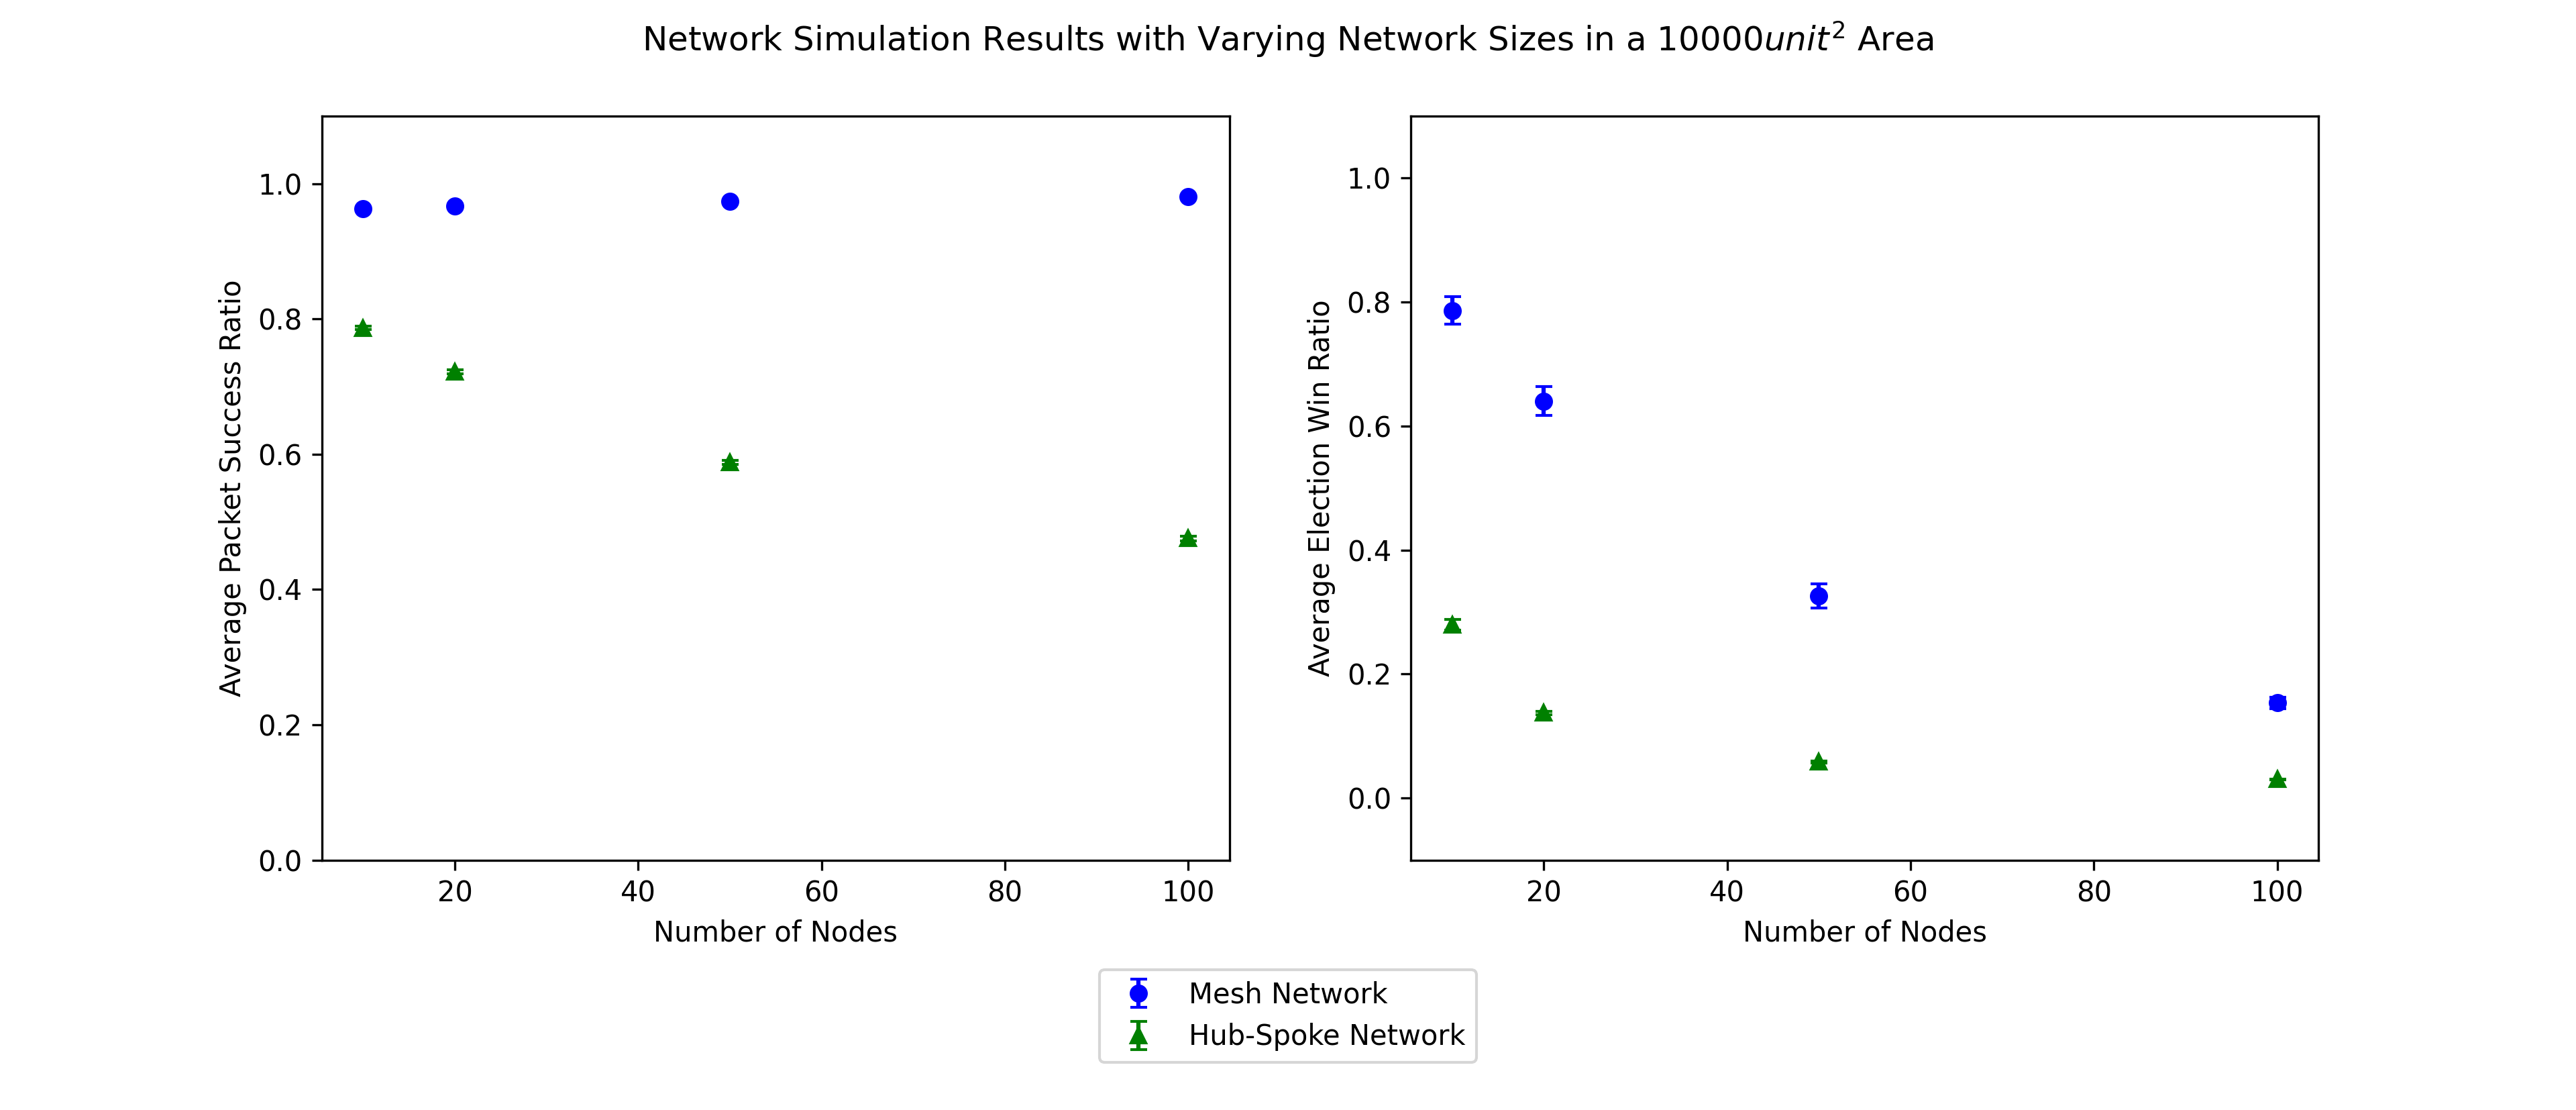
\includegraphics[width=0.9\columnwidth]{images/100unit^2.png}
    \caption{Left: Average packet delivery success ratio per number of nodes, Right: Average ratio of elections won to initiated per number of nodes }
    \label{fig:simulation_result_100}
\end{figure}

Given the results from Figure \ref{fig:simulation_result_100} and those found in Appendix \ref{sec:appendix-for-coracle-results}, we suggest that a mesh network can better recover from abrupt changes to the system, which is characteristic of the dynamic network topologies of mobile systems.

We then used Coracle to further explore mesh networks by varying three main parameters: the number of nodes in the network, the duration between heartbeat messages sent by the consensus leader, and the upper bound of the election timeout. 

Figure \ref{fig:coracle_vary_nodes} shows the average time to first leader (ATFL) and the average ratio of elections won to initiated (AER) for various network sizes ($number\_of\_nodes$ $ = $ $[3,$ $5,$ $10,$ $20,$ $30,$ $50,$ $80,$ $100]$). Here the heartbeat interval was constrained to 30 milliseconds and the election timeout range was set between 60-300 milliseconds.

\begin{figure}[H]
    \centering
    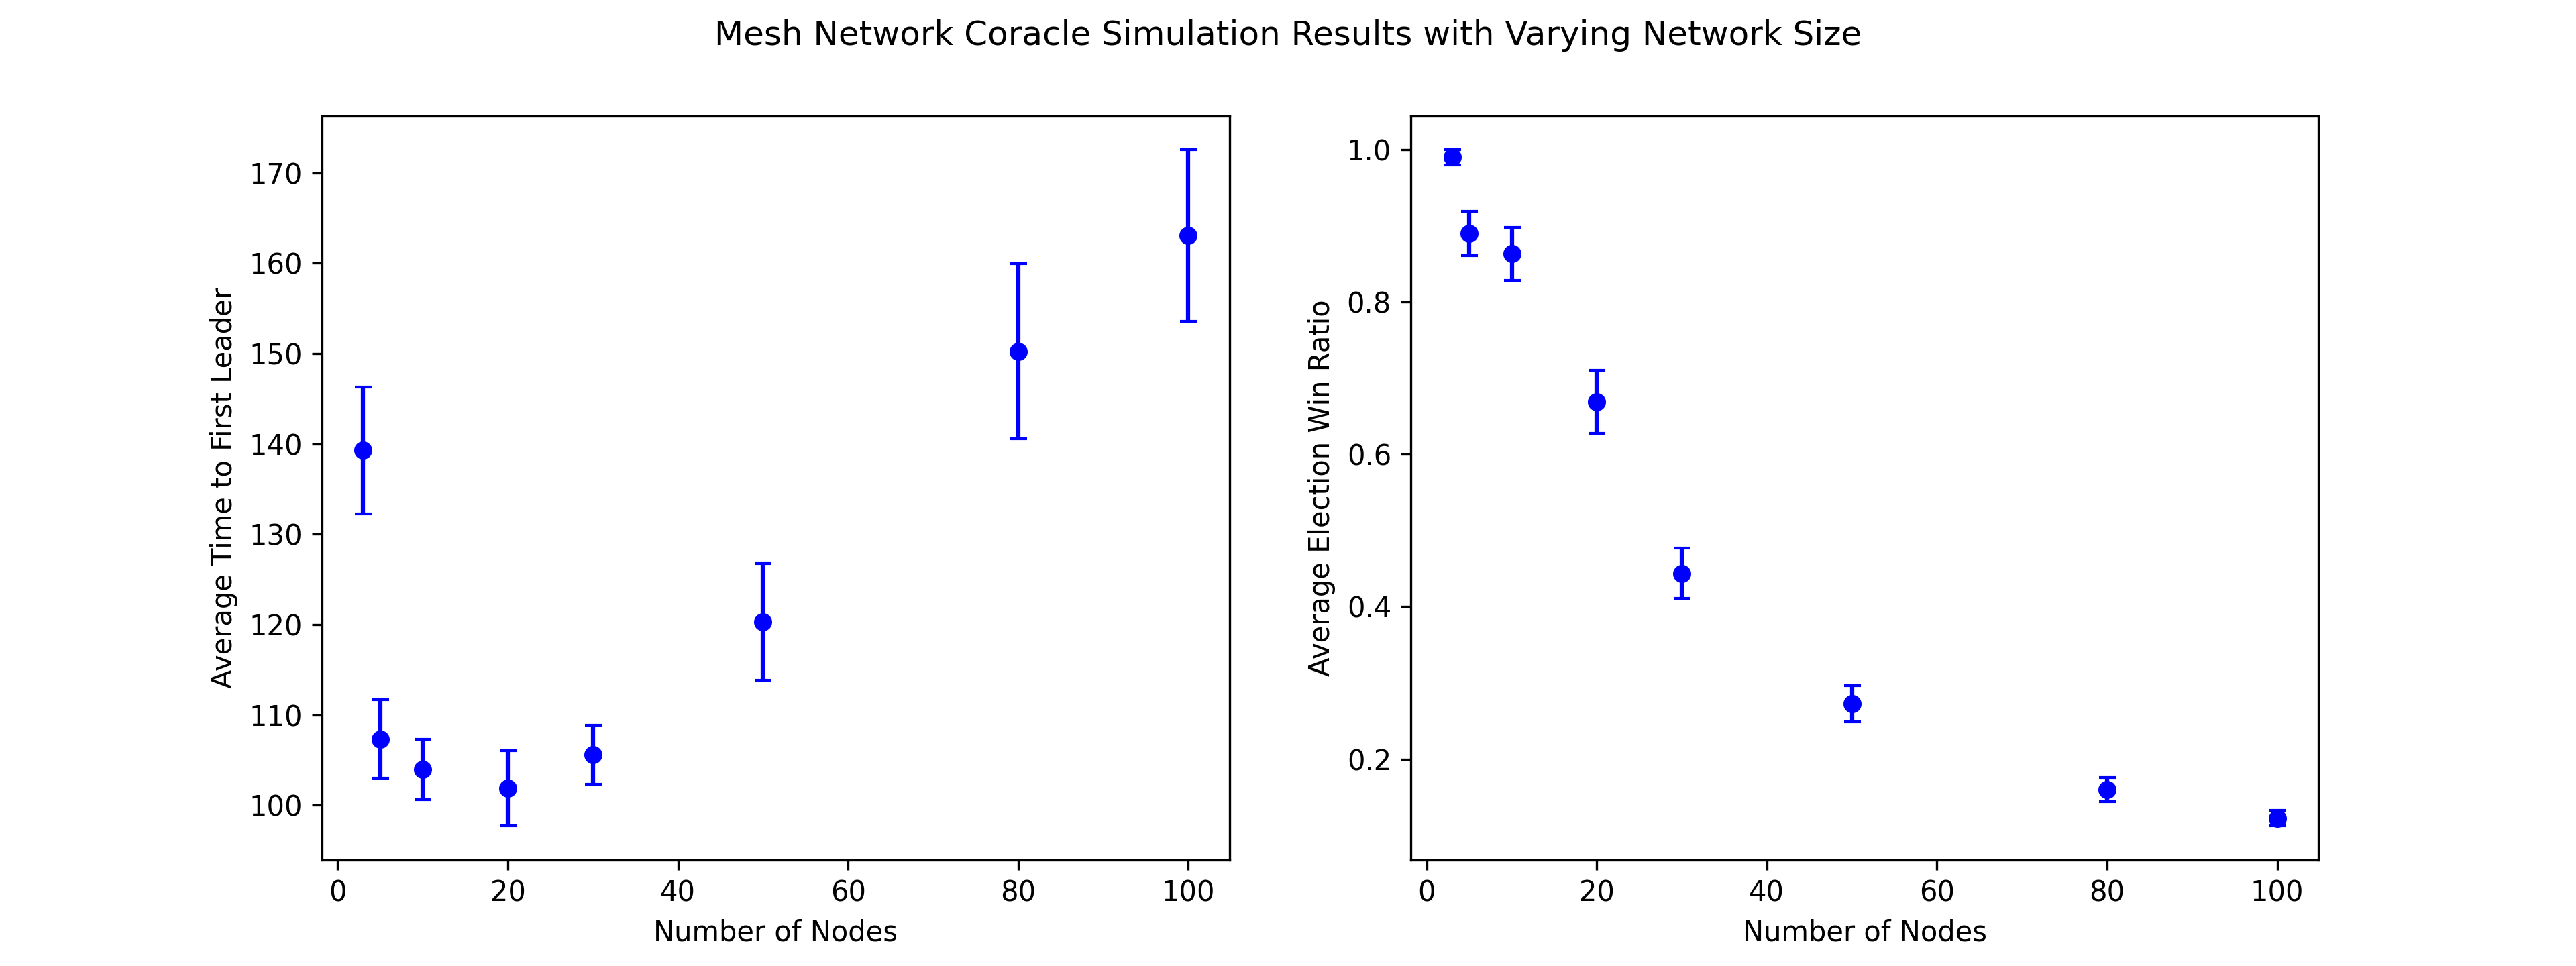
\includegraphics[width=0.9\columnwidth]{images/coracle_vary_nodes.png}
    \caption{Left: Average time to first leader per number of nodes, Right: Average ratio of elections won to initiated per number of nodes}
    \label{fig:coracle_vary_nodes}
\end{figure}

The results clearly indicate that as the number of nodes increase, more elections tend to be wasted. Interestingly, the results also indicate that a network can be too small or too large in coming to an agreement over the selection of a leader. A small network may take too long to gain a majority vote, while a network too large may have difficulty in sending its vote requests out to the other nodes before they time out and start their own elections. 

Figure \ref{fig:coracle_vary_heartbeat} shows the results of varying heartbeat intervals ($heart\_beat\_periods$ $ = $ $[60,$ $120,$ $180,$ $240,$ $300,$ $360,$ $420,$ $480,$ $540,$ $600,$ $660,$ $720]
$) to test for ATFL and AER. In these simulations, the network size was set to 20 nodes and the election timeout range was set between 60-300 milliseconds.

\begin{figure}[H]
    \centering
    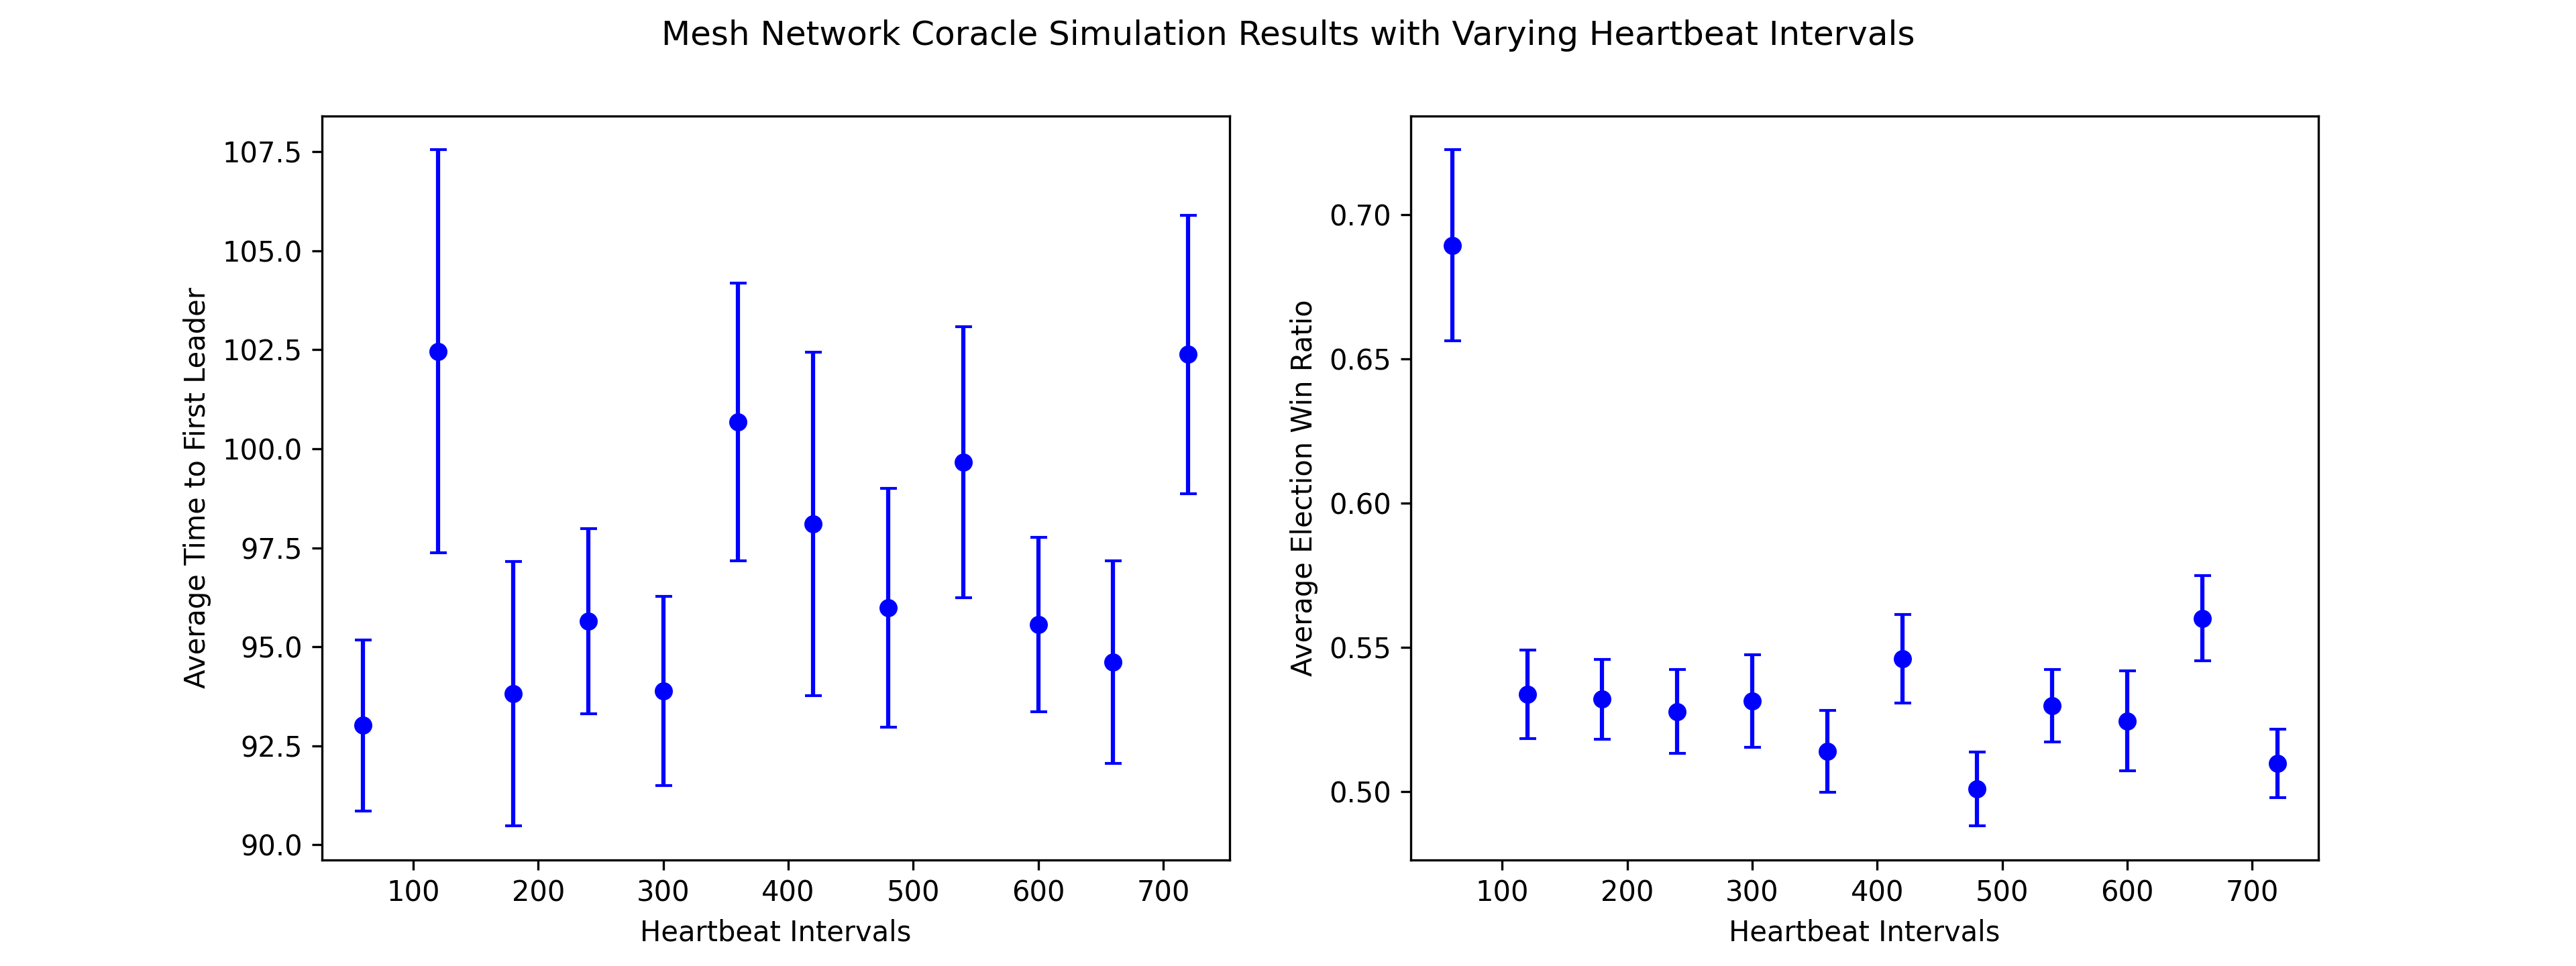
\includegraphics[width=0.9\columnwidth]{images/coracle_vary_heartbeat.png}
    \caption{Left: Average time to first leader per change in heartbeat interval, Right: Average ratio of elections won to initiated per change in heartbeat interval }
    \label{fig:coracle_vary_heartbeat}
\end{figure}

There is no clear answer as to whether varying heartbeat intervals has a significant effect on the ATL; however, 60 milliseconds is clearly the optimal time when looking at AER. Since the difference in AER between a network using 60 milliseconds and 120 milliseconds is so large, we hypothesize that this may actually be a result of how Coracle was implemented and how time is handled in the simulation.

Finally, Figure \ref{fig:coracle_vary_election_timeout} shows the results of varying the upper-bound of the election timeout, effectively increasing the average time it takes for a node to timeout and switch from a follower to a candidate state. Here, the heartbeat interval was fixed to 30 milliseconds while the network size was limited to 20 nodes.

\begin{figure}[H]
    \centering
    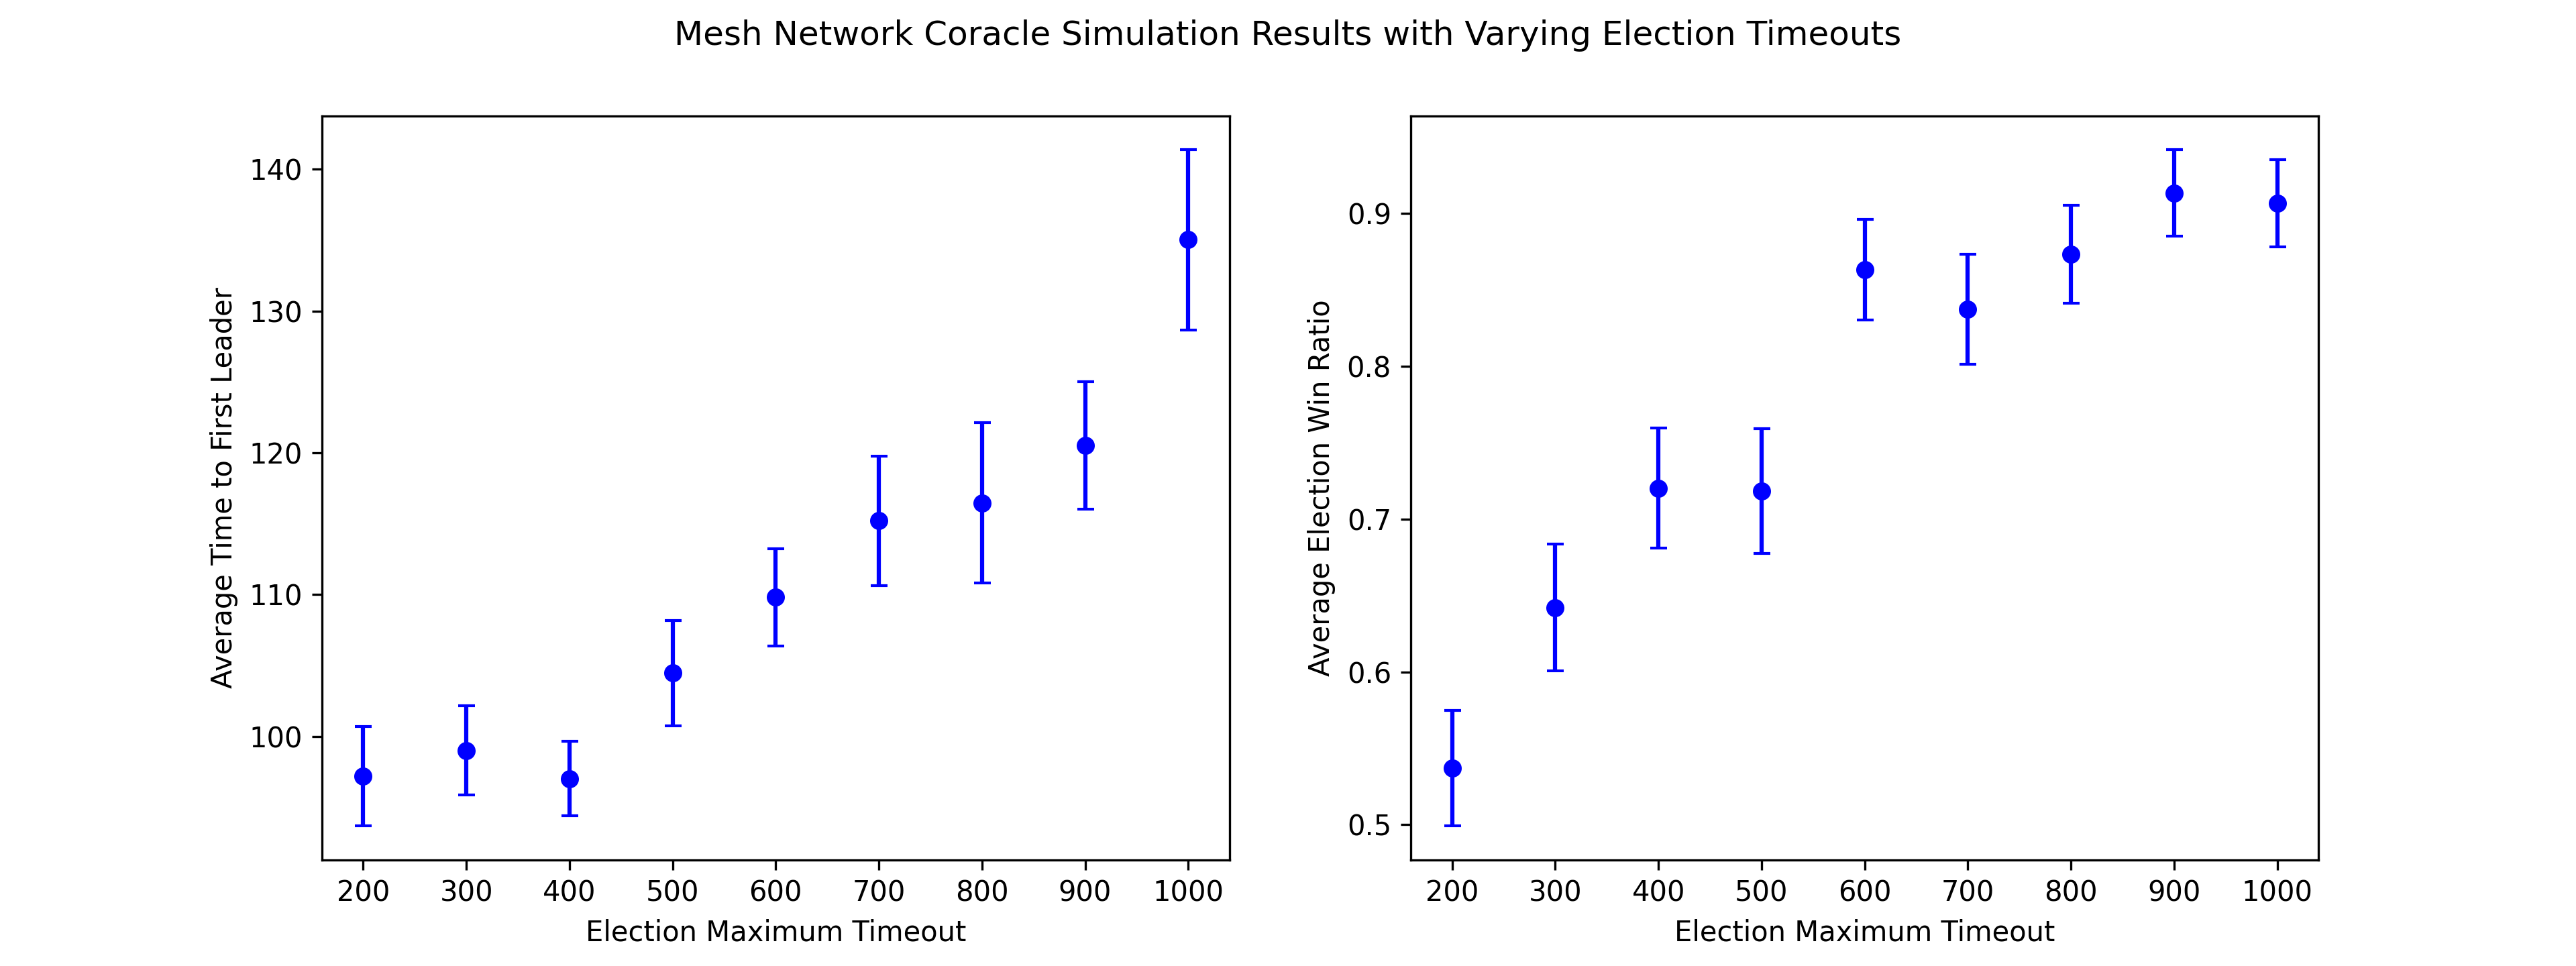
\includegraphics[width=0.9\columnwidth]{images/coracle_vary_election_timeout.png}
    \caption{Left:Average time to first leader per change in maximum possible election timeout, Right: Average ratio of elections won to initiated per change in maximum possible election timeout}
    \label{fig:coracle_vary_election_timeout}
\end{figure}

The results in Figure \ref{fig:coracle_vary_election_timeout} seem to indicate that a large election maximum timeout, which translates to a greater average election timeout, is always better: both the ATL and AER increase as the timeout period increases. However, a large election timeout pushes the network to behave in a more centralized way. A large election timeout would be detrimental to a system where the leader may quickly fall out of the network because the other nodes would be slow to step in for a chance at becoming the leader. Large gaps between leaders will fill the data buffers of the nodes, creating a backlog that could overload the network.

Overall, visualizing how the network reacts to changes in certain parameters helped inform us on how to select the parameters for our implementation. Section \ref{sec:optimization_performed} details how we used these results in our system.

%%%%%%%%%%%%%%%%%%%%%%%%%%%%%%%%%%%%%%%%%%
\subsection{Optimization Performed}
\label{sec:optimization_performed}

We followed the experimental plan below to optimize our software library:
\begin{enumerate}
    \item Using NetworkX and SciKits software libraries, we generated models for star and mesh network topologies in virtual spaces.
    \item We ran Coracle simulations on the network models, adjusting for different parameters such as range, the maximum distance between nodes, maximum concurrent connections, virtual space, election timeouts, heartbeat intervals, and link failure rate.
    \item Informed with the theoretical limitations of Raft and practical limitations of painlessMesh, we wrote our consensus on mesh software library.  
    \item Throughout implementing our software library, we tested modules of the library on ESP8266 development boards and on a virtual network of nodes to obtain satisfactory results.
    \item We designed a virtual testing framework that tested a range of parameters similar to those that worked well in Coracle simulations
    \item We used the results of our virtual testing framework to inform the final configuration of our software library.
\end{enumerate}

The modeling and simulations we performed guided us while making the design choices while implementing our software library. In the Coracle simulations, we defined the resilience of a network by three parameters: average packet delivery rate, the average time to the first leader, and average election win to initiated ratio. In using the simulations, our efforts were focused on understanding the Raft parameters, such as typical election timeout and heartbeat frequency, on maximizing packet delivery and minimizing unnecessary elections. As a result, we gained an understanding of the range of environments in which our physical system will have effective use.